\documentclass{utc-report/utc-report}

\usepackage[hidelinks]{hyperref}
\usepackage{lipsum}
\usepackage{graphicx}
\setlength{\parindent}{0pt}

\UV{SY02} 
\title{UTC LaTeX report}
\author{John \sc{DOE}}

\begin{document}

\maketitlepage

\tableofcontents{}

\pagebreak

\section{Introduction}
\lipsum[1]

\section{System Overview}

\subsection{Autonomous Vehicle}

\begin{figure}[h]
    \centering
    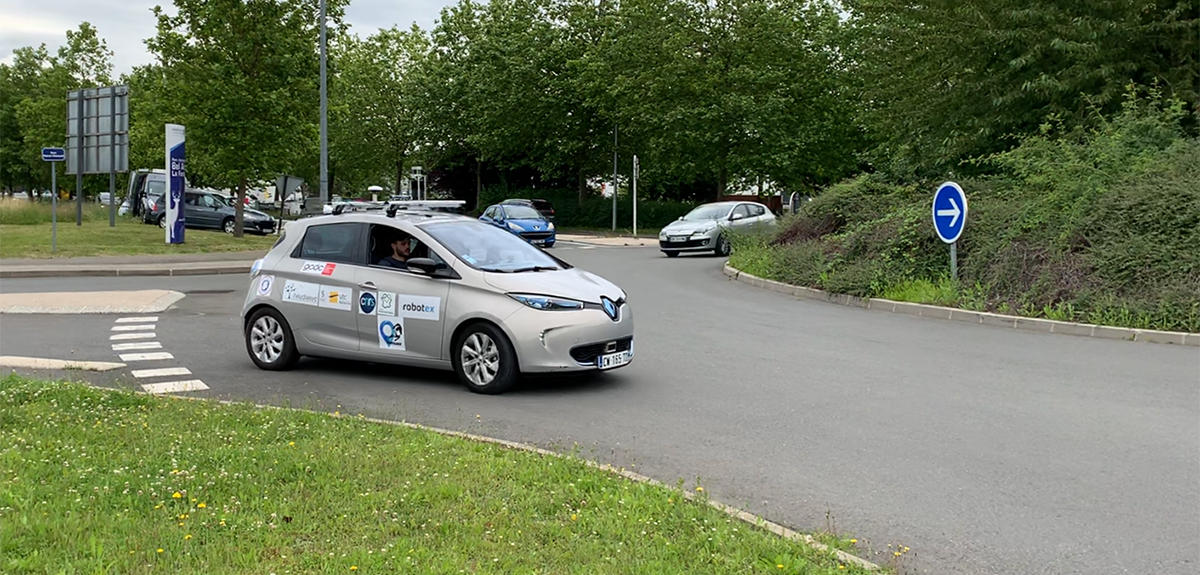
\includegraphics[width=0.7\linewidth]{img/zoe_hds.jpg}
    \caption{Autonomous vehicle of the Heudiasyc laboratory}
\end{figure}

\lipsum[2]

\pagebreak

\subsection{Scheduling Constraints}

\subsubsection*{Availability}

Each task can only start after its release date:

\[
    T_i \geq r_i \quad \forall i \in \{1, 2, 3, 4, 5\}.
\]

\subsubsection*{Deadline}

Each task must be completed before its deadline:

\[
    T_i + p_i \leq d_i \quad \forall i \in \{1, 2, 3, 4, 5\}.
\]

\subsubsection*{Non-overlapping}

For any pair of tasks \( J_i \) and \( J_j \) with \( i \neq j \), task \( J_j \) must not start within the execution interval of task \( J_i \). This is expressed as:

\[
    \forall i, j \in \{1, 2, 3, 4, 5\}, \, i \neq j, \quad T_j \notin [T_i, T_i + p_i].
\]

\end{document}
